\section{Scientists: Charles Darwin}
% To illustrate the importance of how to present your
% Research results, let's talk about one researcher
% whose research was all about collecting and displaying data,
% Charles Darwin

\begin{frame}{Charles Darwin}{1809--1882 British Naturalist, Geologist, Biologist}
  To open our discussion about data, let's talk about a scientist whose work was all about collecting and understanding lots of data.
  \bigskip

  \begin{columns}
    \column{.2\textwidth}
    \includegraphics[width=1\textwidth]{../img/irasutoya_darwin}
    \ppagenote{Charles Darwin sketch from \url{https://www.irasutoya.com}}
    \column{.8\textwidth}
    \begin{itemize}
      \item Well known for his theory on \structure{the origin of species}
      \item His theory correctly predicted the hereditary nature of evolution, even before genes were known.
      \item Actually, in his period, many people were interested in understanding the origin of the species;
    \end{itemize}
  \end{columns}
\end{frame}

\begin{frame}{Charlis Darwin}{Early Life}
  % Image: Child Darwin, wikipedia
  \hfill\includegraphics[width=.2\textwidth]{../img/wikipedia_darwinchild}
  \ppagenote{Charles Darwing Portrait from wikipedia (Public Domain)}
  \bigskip

  \begin{itemize}
    \item Son of a wealthy doctor in a large family;
    \item Apprenticed as a doctor, but found the classes dull.
    \item Prefered to learn \structure{taxidermy}, and catalog animals;
  \end{itemize}
\end{frame}

\begin{frame}{Charles Darwin}{Observing the World}
  % Image - HMS Beagle trip, wikipedia
  \begin{itemize}
    \item 1831: After graduation, went on a 5 year sea voyage to catalog geological and animal samples in South America and Asia;\medskip

    \item During the trip, he kept extensive notes of his observations and theories;\medskip

    \item His observations about the diversity of mockingbirds, tortoises, and foxes gave him new insights about the origin of the species;
  \end{itemize}\bigskip

  \begin{center}
    \includegraphics[width=.6\textwidth]{../img/wikipedia_darwin_beagle}
  \end{center}
\end{frame}

\begin{frame}{Charles Darwin}{On the Origin of the Species}
  % Image: The origin of the species
  \begin{columns}
    \column{0.2\textwidth}
    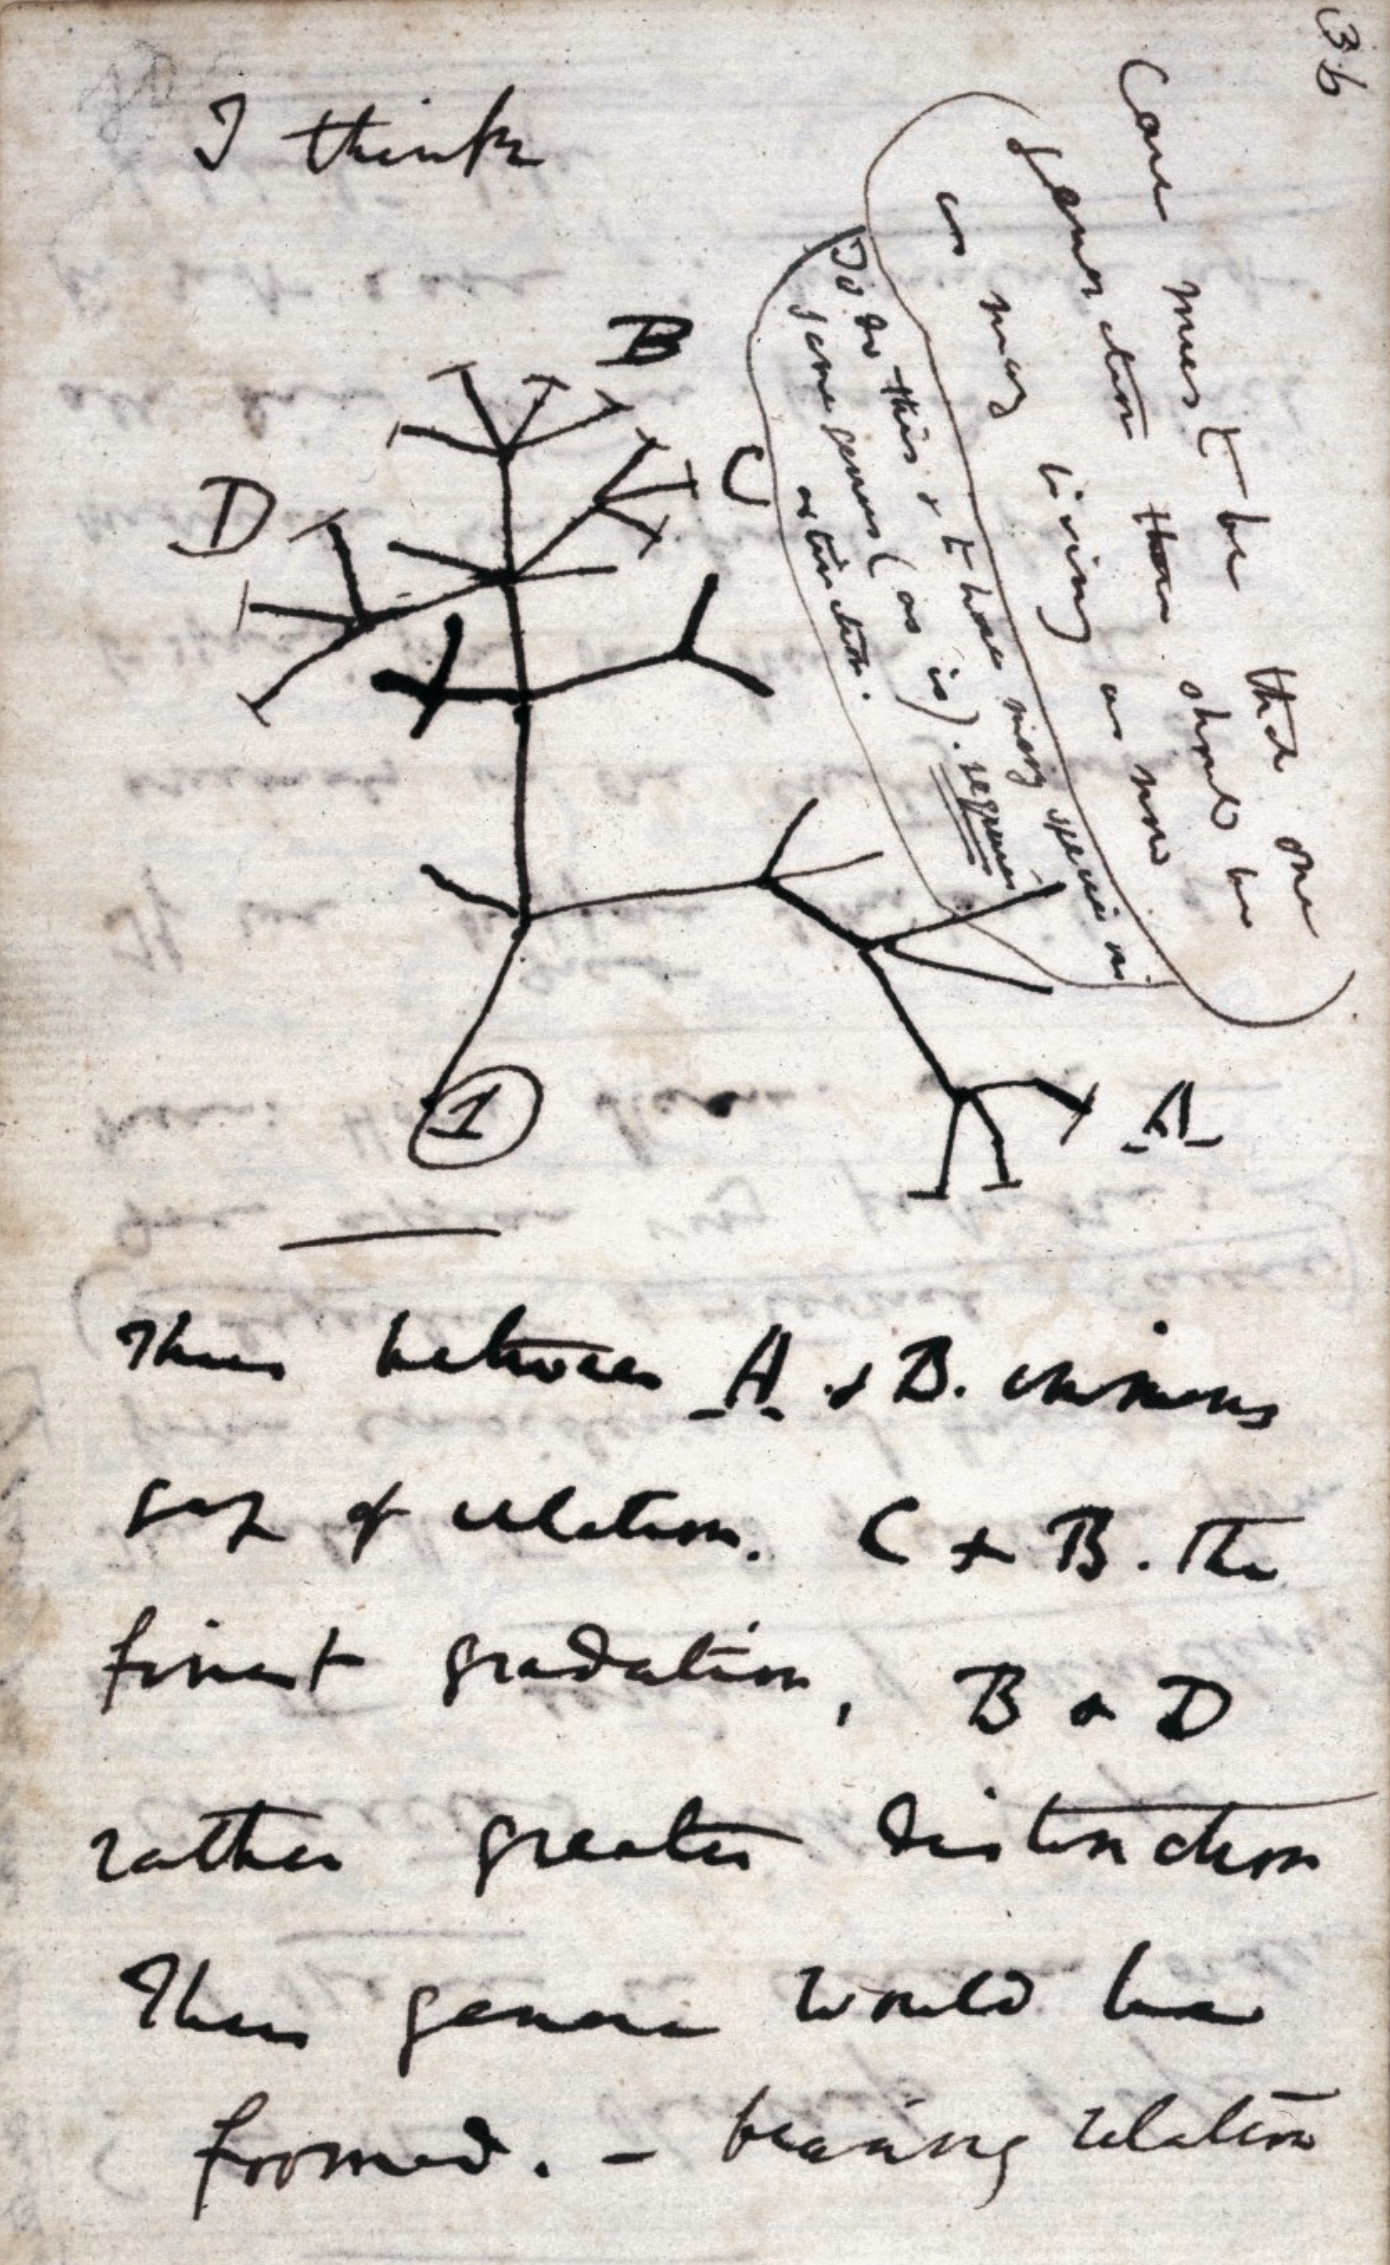
\includegraphics[width=1\textwidth]{../img/wikipedia_darwin_manuscript}
    \column{0.8\textwidth}
  \begin{itemize}
    \item In 1837, his notes from the Beagle's trip gave him his first insights about how "one species transforms into another"
    \item He gathered more and more data to confirm his theory, from marine biologists, farmers and breeders, plants, etc.
    \item This task of cataloguing and experimenting took over 15 years;
    \item Eventually published "On The Origin of the Species" in 1859, by encouragement from his friend scientists;
  \end{itemize}
  \end{columns}
\end{frame}
